\chapter{Взаимодействие h-BN/Co(0001) с молекулярным кислородом} \label{chapt3}

Теоретические исследования показывают, что взаимодействие монослоя гексагонального 
нитрида бора с кислородом приводит к изменению электронных и магнитных
свойств материала~\cite{Ataca2010,Zhou2010}. Важным обстоятельством является то, каким именно образом кислород
вступает во взаимодействие с монослоем h-BN, а именно: встраиваются атомы кислорода в решетку 
h-BN, или интеркалируют под монослой, не образуя связей с ним, или же являются 
адатомами на поверхности монослоя. Таким образом, в данной работе был 
исследован механизм взаимодействия молекулярного кислорода с монослоем h-BN, выращенного на 
поверхности кобальта Co(0001). Посредством серии экспериментов на Российско-Германском
канале вывода СИ синхротрона BESSY II в Берлине были получены экспериментальные 
данные XPS, NEXAFS, а так же ДМЭ. Результаты и выводы по полученным данным 
представлены в данной работе.

\section{Характеристика структуры образца}

После формирования гексагонального нитрида бора на поверхности кобальта, для контроля
качества  поверхности, была получена картина дифракции медленных электронов
рис.~\ref{pic:LEED}. Постоянные решеток Co(0001) и h-BN совпадают, 
	\begin{figure}[!ht]
		\center{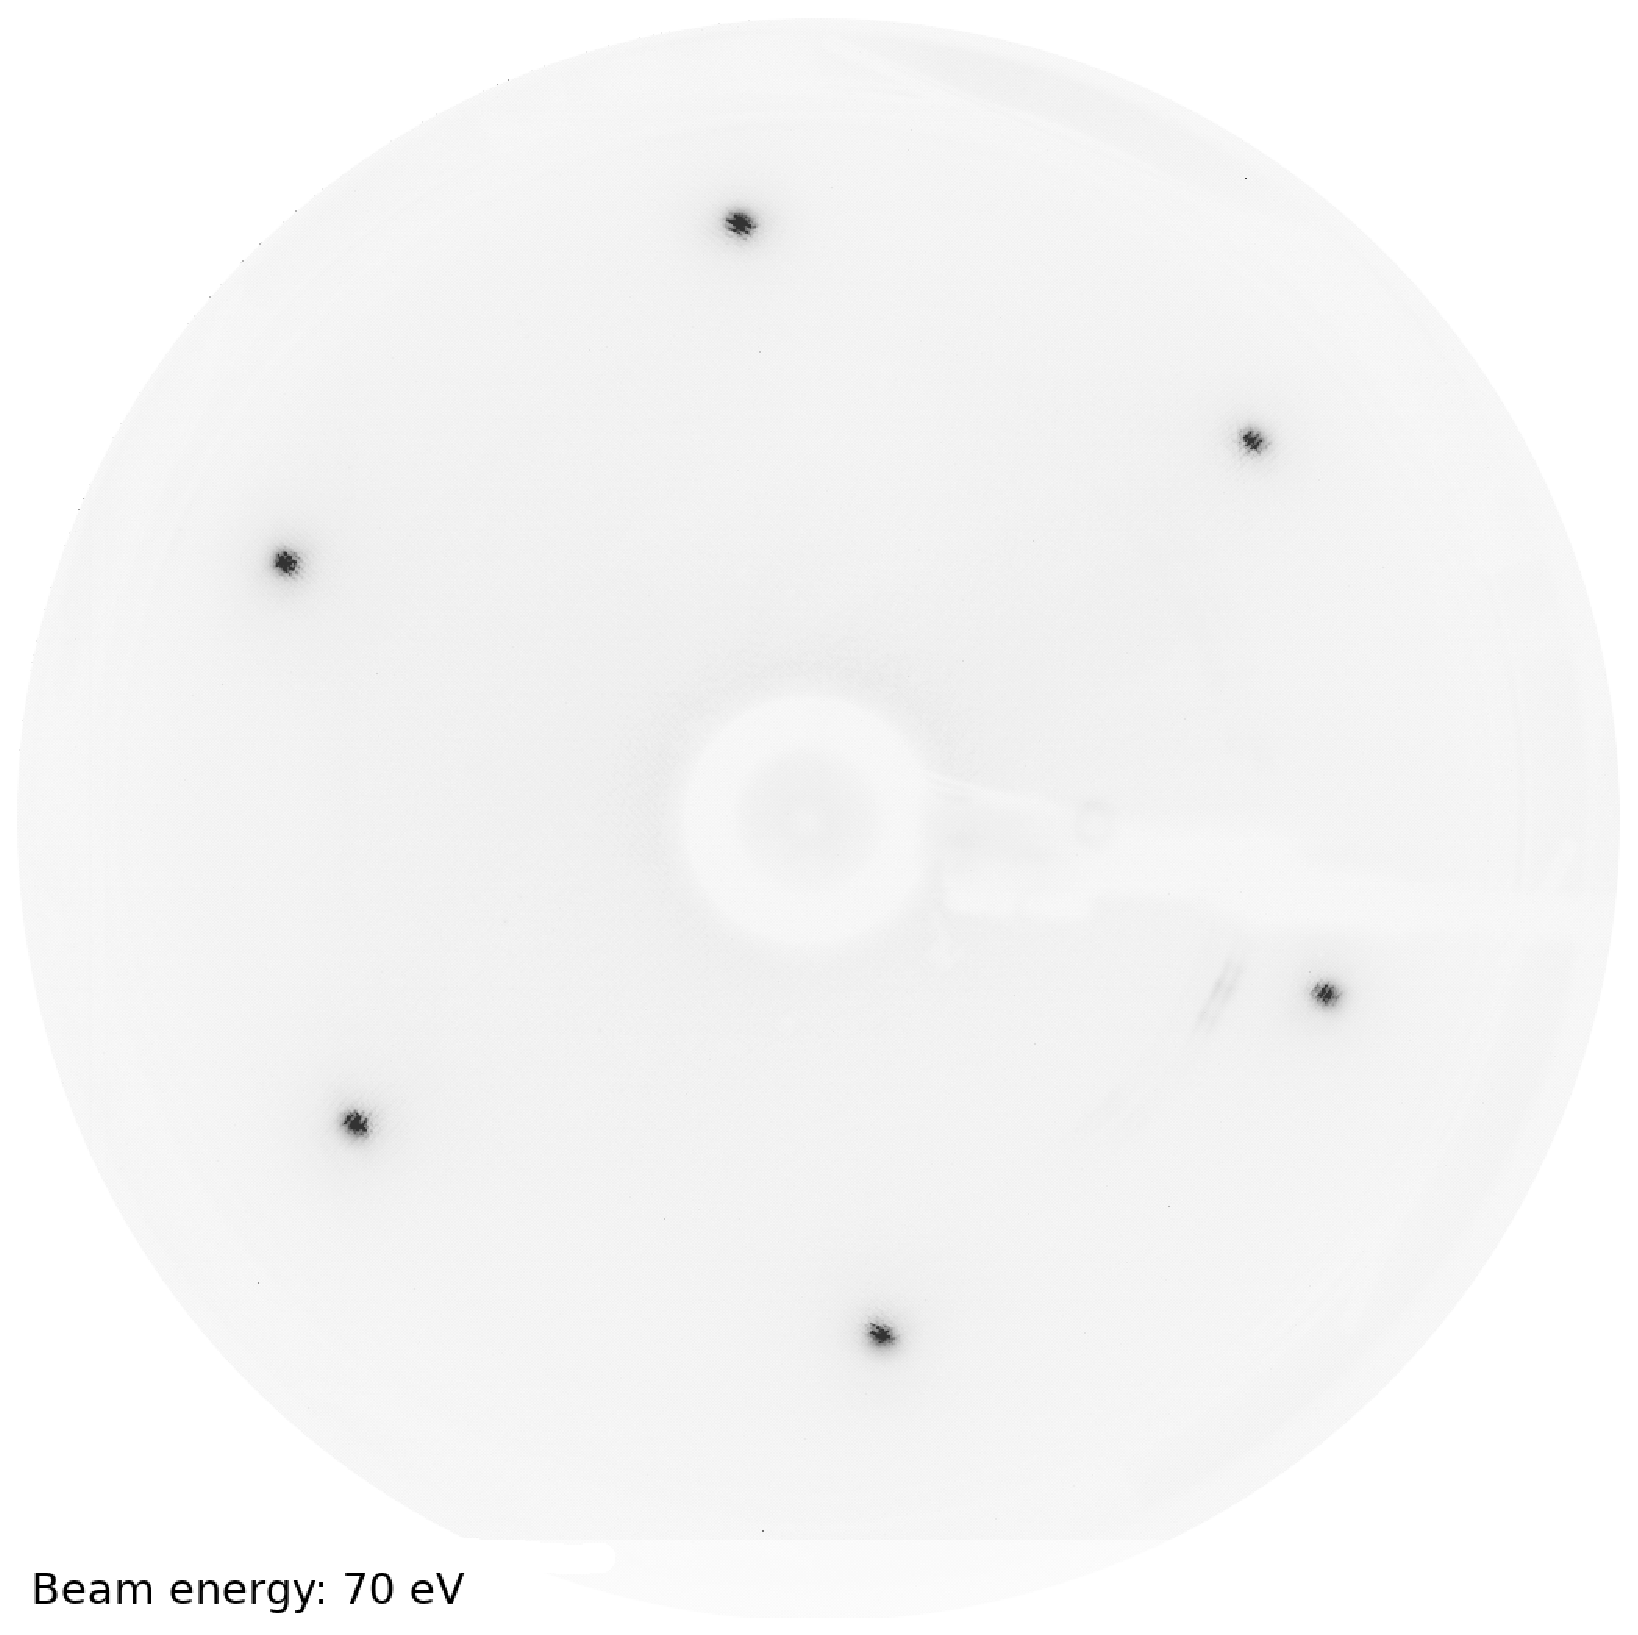
\includegraphics[width=0.3\linewidth]{LEED.eps}}
		\caption{ДМЭ картина соответствующая поверхностной фазе h-BN/Co(0001)($E_p = 70 eV$).}
		\label{pic:LEED}
	\end{figure}
этому свидетельствует четко выраженная гексагональная структура $(1\times1)$ 
и отсутствие расщепления рефлексов.
Это говорит о том, что выращенный кристалл h-BN строго
ориентирован относительно подложки.



\section{Экспериментальные спектры и их обсуждение}

Полученная система h-BN/Co(0001) прогревалась в атмосфере
кислорода. Прогрев производился поэтапно при давлении молекулярного кислорода $10^{-5}$ мбар и при температуре 300\degree C. Эти параметры выбраны 
таким образом, чтобы заметные изменения в системе происходили за времена
порядка десятков минут:
	\vspace{15pt}
		\begin{enumerate}
			\item Первый шаг. Прогрев системы h-BN/Co(0001) под давлением $10^{-5}$ мбар в течение 10 минут.
			\item Второй шаг. Прогрев системы h-BN/Co(0001) под давлением $10^{-5}$ мбар в течение 10 минут.
			\item Третий шаг. Прогрев системы h-BN/Co(0001) под давлением $10^{-5}$ мбар в течение 10 минут.
			\item Четвертый шаг. Прогрев системы h-BN/Co(0001) под давлением $10^{-5}$ мбар в течение 10 минут.
			\item Пятый шаг. Прогрев системы h-BN/Co(0001) под давлением $10^{-5}$ мбар в течение 10 минут.
			\item Шестой шаг. Прогрев системы h-BN/Co(0001) под давлением $10^{-5}$ мбар в течение 30 минут.
			\item Седьмой шаг. Прогрев системы h-BN/Co(0001) под давлением $10^{-5}$ мбар в течение 60 минут.
		\end{enumerate}
	\vspace{15pt}
Таким образом, суммарное время прогрева системы h-BN/Co(0001) в кислороде составило 140 минут.
На каждом этапе снимались РФЭС и NEXAFS спектры.
Далее в работе представленны результаты обработки и анализа полученных спектров.



\subsection{Анализ фотоэлектронных спектров}

На рис.~\ref{pic:Surveys} представлена серия фотоэлектронных спектров поверхности h-BN/Co(0001).
Каждый спектр соответствует этапу прогрева образца в кислороде. Таким образом, первый спектр характеризует
поверхность до прогрева в кислороде, а последний -- после 140 минут. Видно, что вначале
	\begin{figure}[!ht]
		\center{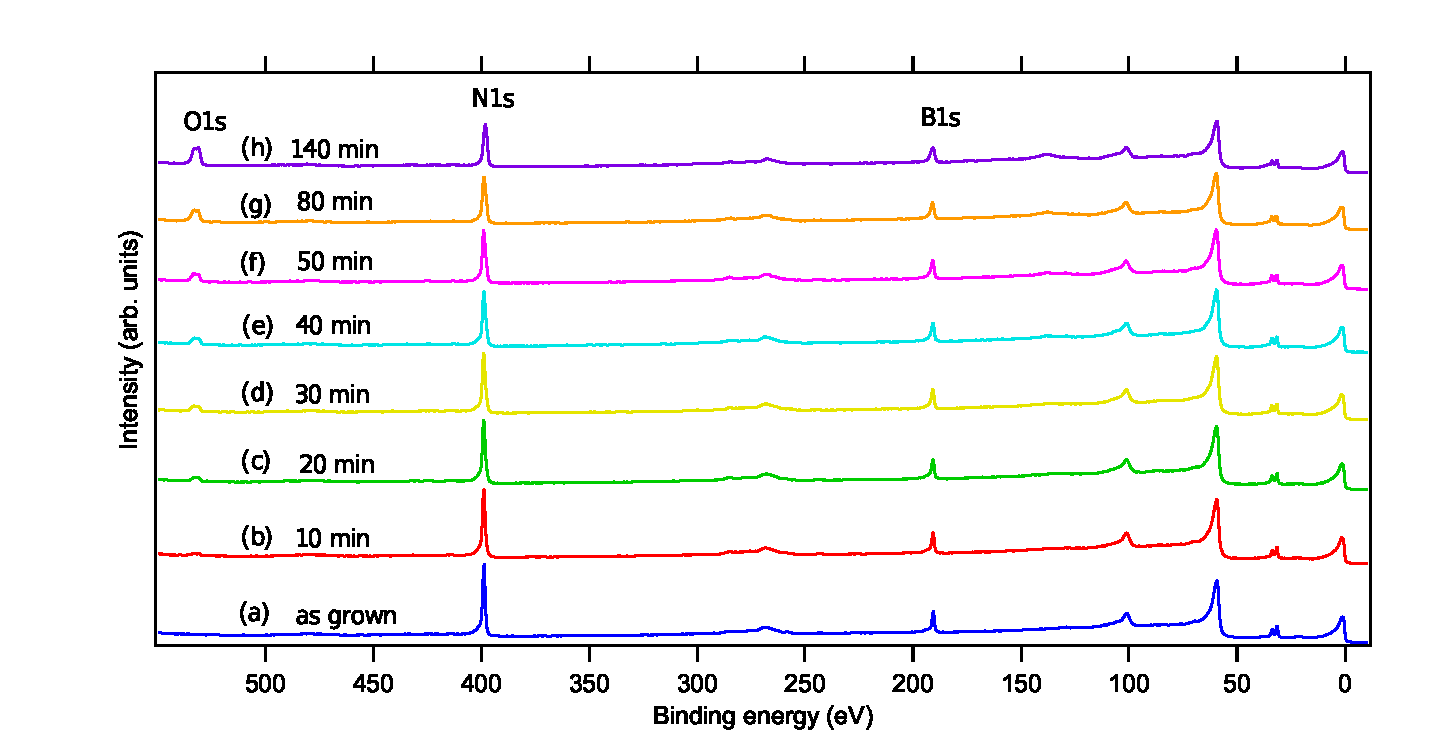
\includegraphics[width=1\linewidth]{Surveys}}
		\caption{Обзорные фотоэлектронные спектры h-BN/Co(0001) в процессе прогрева в кислороде, записанные с энергией
		возбуждающих квантов 650 eV}
		\label{pic:Surveys}
	\end{figure}
отсутствует пик кислорода O1s, который появляется уже на первом этапе после 10 минут 
прогрева h-BN/Co(0001) в кислороде, и растет со временем. Также можно заметить, что пик 
интенсивности азота N1s убывает в течение прогрева, в то время как пик 
интенсивности бора B1s остается неизменным. Зависимость концентраций азота, бора и кислорода 
в атомарных процентах на поверхности системы
h-BN/Co(0001) от времени представлена на рис.~\ref{pic:B_N_O_tot_percent}. За 100~ат\% было принято
полное количество атомов азота и бора в монослое h-BN.
На чистой поверхности образца кислород отсутствует, а на бор с азотом приходится
по 50~ат\% концентрации. Далее, с прогревом h-BN/Co(0001) в кислороде, концентрация кислорода увеличивается
и доходит до отметки в 14.9~ат\%. В процессе экспозиции концентрация азота уменьшается на 8.5~ат\%.
Концентрация бора остается постоянной. Представленные зависимости демонстрируют, что количество 
азота в кристаллической решетке гексагонального нитрида бора убывает, а кислорода возрастает.
Такое же поведение системы h-BN/Ir(111) при окислении наблюдалось в работе~\cite{Simonov2012_h-BN/Ir_Oxydation}. 
	\begin{figure}[!ht]
		\center{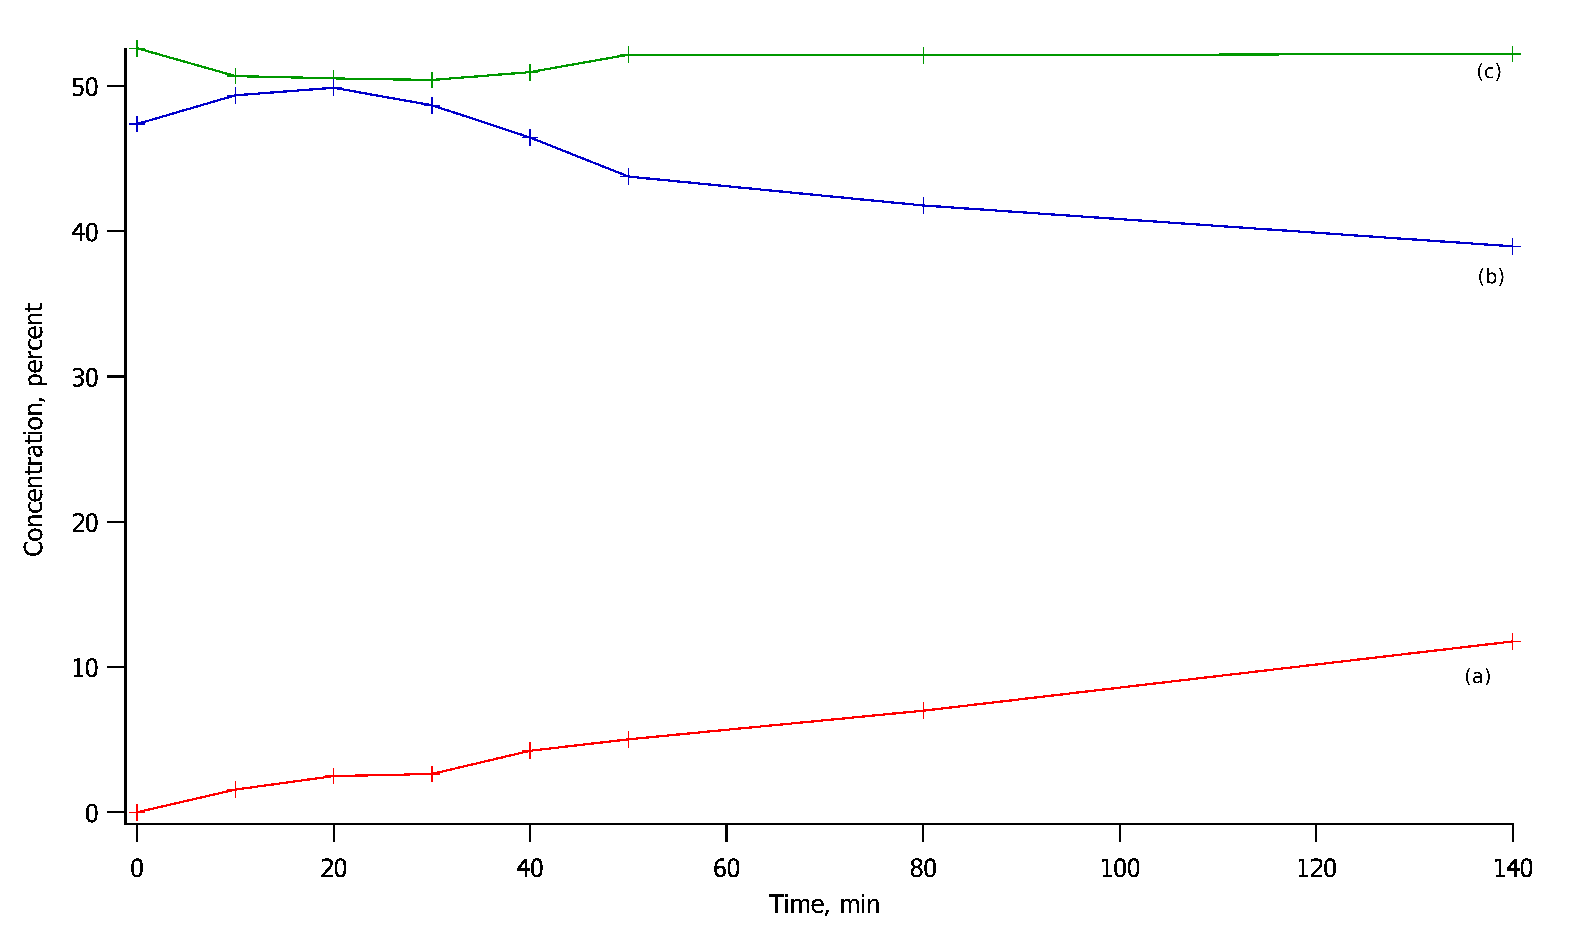
\includegraphics[width=0.8\linewidth]{N_B_O_tot_percent_vs_time}}
		\caption{Зависимость концентраций от времени (a) бора, (b) азота, (c) кислорода.}
		\label{pic:B_N_O_tot_percent}
	\end{figure}
Здесь можно сделать предположение, что атомы кислорода встраиваются в кристаллическую решетку
нитрида бора, замещая атомы азота.


Далее мы рассмотрели пики интенсивностей B1s, N1s и O1s по отдельности и пронаблюдали их эволюцию
от первого этапа с чистой поверхностью до последнего этапа после 140 минут экспозиции системы h-BN/Co(0001) в кислороде. 
На рис.~\ref{pic:B1s_N1s} представлены пики интенсивностей фотоэмиссии B1s и N1s.
	\begin{figure}[!ht]
		\center{\includegraphics[width=0.8\linewidth]{B1s_N1s_fits.eps}}
		\caption{РФЭС линии (i) B1s-, (ii) N1s-уровней от исходного h-BN (as grown) и на разных стадиях окисления.}
		\label{pic:B1s_N1s}
	\end{figure}
Пик $\mathrm{b_1}$ на рисунке~\ref{pic:B1s_N1s}(i) с энергией связи 190.4 eV соответствует основному пику 
чистого h-BN сильно связанного с Co(0001)~\cite{Usachov2018_h-BN/_PED_STM}. Уже после 10 минут прогрева системы в кислороде появляется два пика
$\mathrm{b_2}$ с энергией связи 191.3 eV и $\mathrm{b_3}$ с энергией связи 190.2 eV. Пик $\mathrm{b_3}$  имеет меньшую энергию связи. Такое появление пика интенсивности в области более низкой энергии связи может быть
связано с интеркаляцией кислорода под монослой h-BN, так, например, в работе~\cite{Usachov2017_Graphen_RS}
интеркаляция кислорода под монослой графена в системе graphen/Co(0001) тоже сопровождалась химическим сдвигом пика C1s. Пик $\mathrm{b_2}$, 
относительно $\mathrm{b_1}$, сдвинут в область больших энергий связи. Химический сдвиг в область увеличения энергии связи может быть обусловлен
образованием связи $\mathrm{B-O}$~\cite{Petravic2010}. Пик $\mathrm{b_2}$ появляется в результате встраивания кислорода
в решетку гексагонального нитрида бора с замещением атома азота на атом кислорода и образованием локальной структуры 
$\mathrm{BN_2O}$~\cite{Makarova2019_h-BN/Ni_Oxydation}.
Компонента $\mathrm{b_4}$ появляется только после 40 минут экспозиции и может
быть связана с образованием $\mathrm{BO_3}$, где уже все три атома азота замещены атомами кислорода. После 140 минут прогревания системы 
h-BN/Co(0001) пик $\mathrm{b_1}$ теряет свою интенсивность, а пики $\mathrm{b_2}$ и $\mathrm{b_3}$ становятся преобладающими. Это говорит 
нам о том, что на поверхности h-BN преимущественно образуются оксидные группы $\mathrm{BN_2O}$.
	\begin{figure}[!ht]
		\center{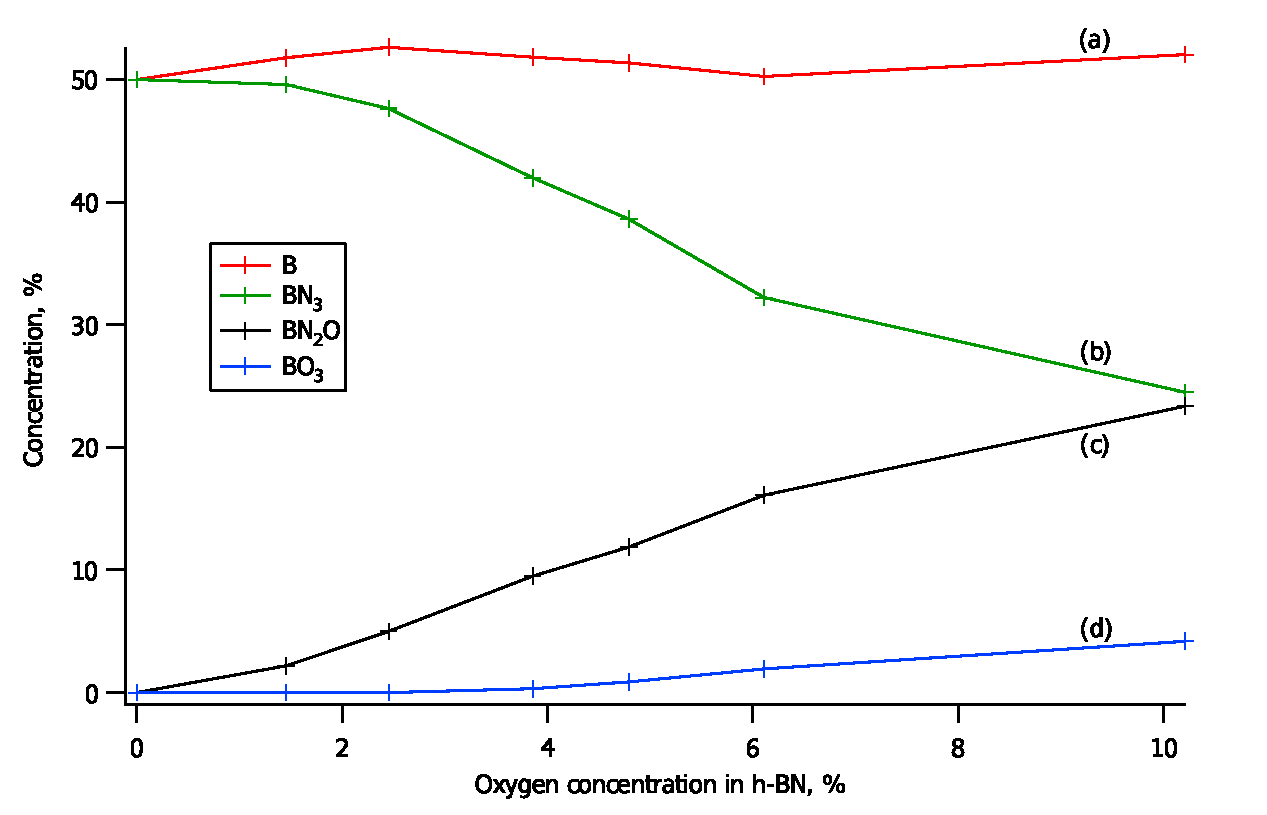
\includegraphics[width=0.8\linewidth]{Concentration_B_BN3_BN2O_BO3_vs_O.eps}}
		\caption{График зависимости концентраций B (a), $\mathrm{BN_3}$ (b), $\mathrm{BN_2O}$ (c) и $\mathrm{BO_3}$ (d) от концентрации молекулярного кислорода, встроенного в решетку гексагонального нитрида бора.}
		\label{pic:B_BN3_BN2O_BO3_vs_O}
	\end{figure}


На рис.~\ref{pic:B_BN3_BN2O_BO3_vs_O} представлен график зависимости концентраций всего бора B (a), бора, связанного с Co(0001)
$\mathrm{BN_3}$ (b), бора, связанного с одним атомом кислорода $\mathrm{BN_2O}$ (c), и бора, связанного с тремя атомами кислорода
$\mathrm{BO_3}$ (d), от концентрации кислорода, встроенного в решетку гексагонального нитрида бора. Концентрация бора (a) на поверхности
остается неизменна на протяжении всего времени экспозиции. Концентрация бора, сильно связанного с подложкой кобальта (b), характерно 
уменьшается и к седьмому этапу экспозиции с 50~ат\% убывает до 24,5~ат\%. Концентрация структуры $\mathrm{BN_2O}$, появляющейся уже после
первого этапа прогревания системы h-BN/Co(0001), растет в течение всего эксперимента и к последнему этапу возрастает до 23.3~ат\%. 
Структура $\mathrm{BO_3}$ появляется только после 40 минут экспозиции, а ее концентрация на последнем этапе доходит до отметки 4.1~атомовт\%. Таким образом, можно
сделать вывод, что с увеличением концентрации атомов кислорода в решетке h-BN, преимущественно образуются структуры вида
$\mathrm{BN_2O}$, при этом атомы бора не покидают системы h-BN/Co(0001).


На рис.~\ref{pic:B1s_N1s}(ii) представлена серия фотоэмиссионных спектров азота N1s, полученных на различных этапах прогрева h-BN/Co(0001) в кислороде.
Пик $\mathrm{n_1}$ с энергией связи 398.5 eV соответствует основному пику чистого h-BN сильно связанного с Co(0001).После 10 минут экспозиции в пике азота появляются две новые компоненты $\mathrm{n_2}$ с энергией связи 397.7 eV и $\mathrm{n_3}$ с энергией связи 397.2 eV. Энергия связи этих двух пиков меньше, чем у пика $\mathrm{n_1}$. Как было отмечено выше, такой химический сдвиг может быть результатом интеркаляции атомов кислорода под монослой h-BN. Наличие двух пиков с разным химическим сдвигом в сторону меньших энергий связи можно объяснить разным количеством  атомов кислорода под атомами азота. Общая интенсивность пика N1s в течение экспозиции уменьшается, что является следствием уменьшения количества азота в структуре h-BN/Co(0001). Другими словами, происходит десорбция атомов азота, замещенных атомами кислорода.
	\begin{figure}[!ht]
		\center{\includegraphics[width=0.8\linewidth]{Conc_Nfree_Nco_Ntot_vs_O.eps}}
		\caption{График зависимости концентраций всего азота (a), азота связанного с Co(0001) (b) и азота несвязанного с подложкой (c) и (d) от концентрации кислорода, встроенного в решетку h-BN.}
		\label{pic:Nfree_Nco_Ntot_vs_O}
	\end{figure}


Зависимость концентраций пиков азота от концентрации кислорода, встроенного в решетку гексагонального нитрида бора
представлена на рис.~\ref{pic:Nfree_Nco_Ntot_vs_O}. Кривая (a) соответствует концентрации азота на поверхности
h-BN/Co(0001). Убывание этой кривой свидетельствует о том, что, с увеличением количества атомов кислорода в решетке монослоя h-BN,
количество атомов азота уменьшается. Азоту, сильно связанному с Co(0001), соответствует 
кривая (b). Она характерно убывает с ростом концентрации кислорода, в то время как кривые (c) и (d) растут. Кривые (c) и (d) отвечают азоту, слабо связанному с подложкой кобальта в результате интеркаляции кислорода. Такое поведение 
кривых концентраций говорит о том что, вместе с процессом встраивания кислорода в решетку h-BN, так же происходит интеркаляция атомов кислорода под монослой гексагонального нитрида бора.
	\begin{figure}[!ht]
		\center{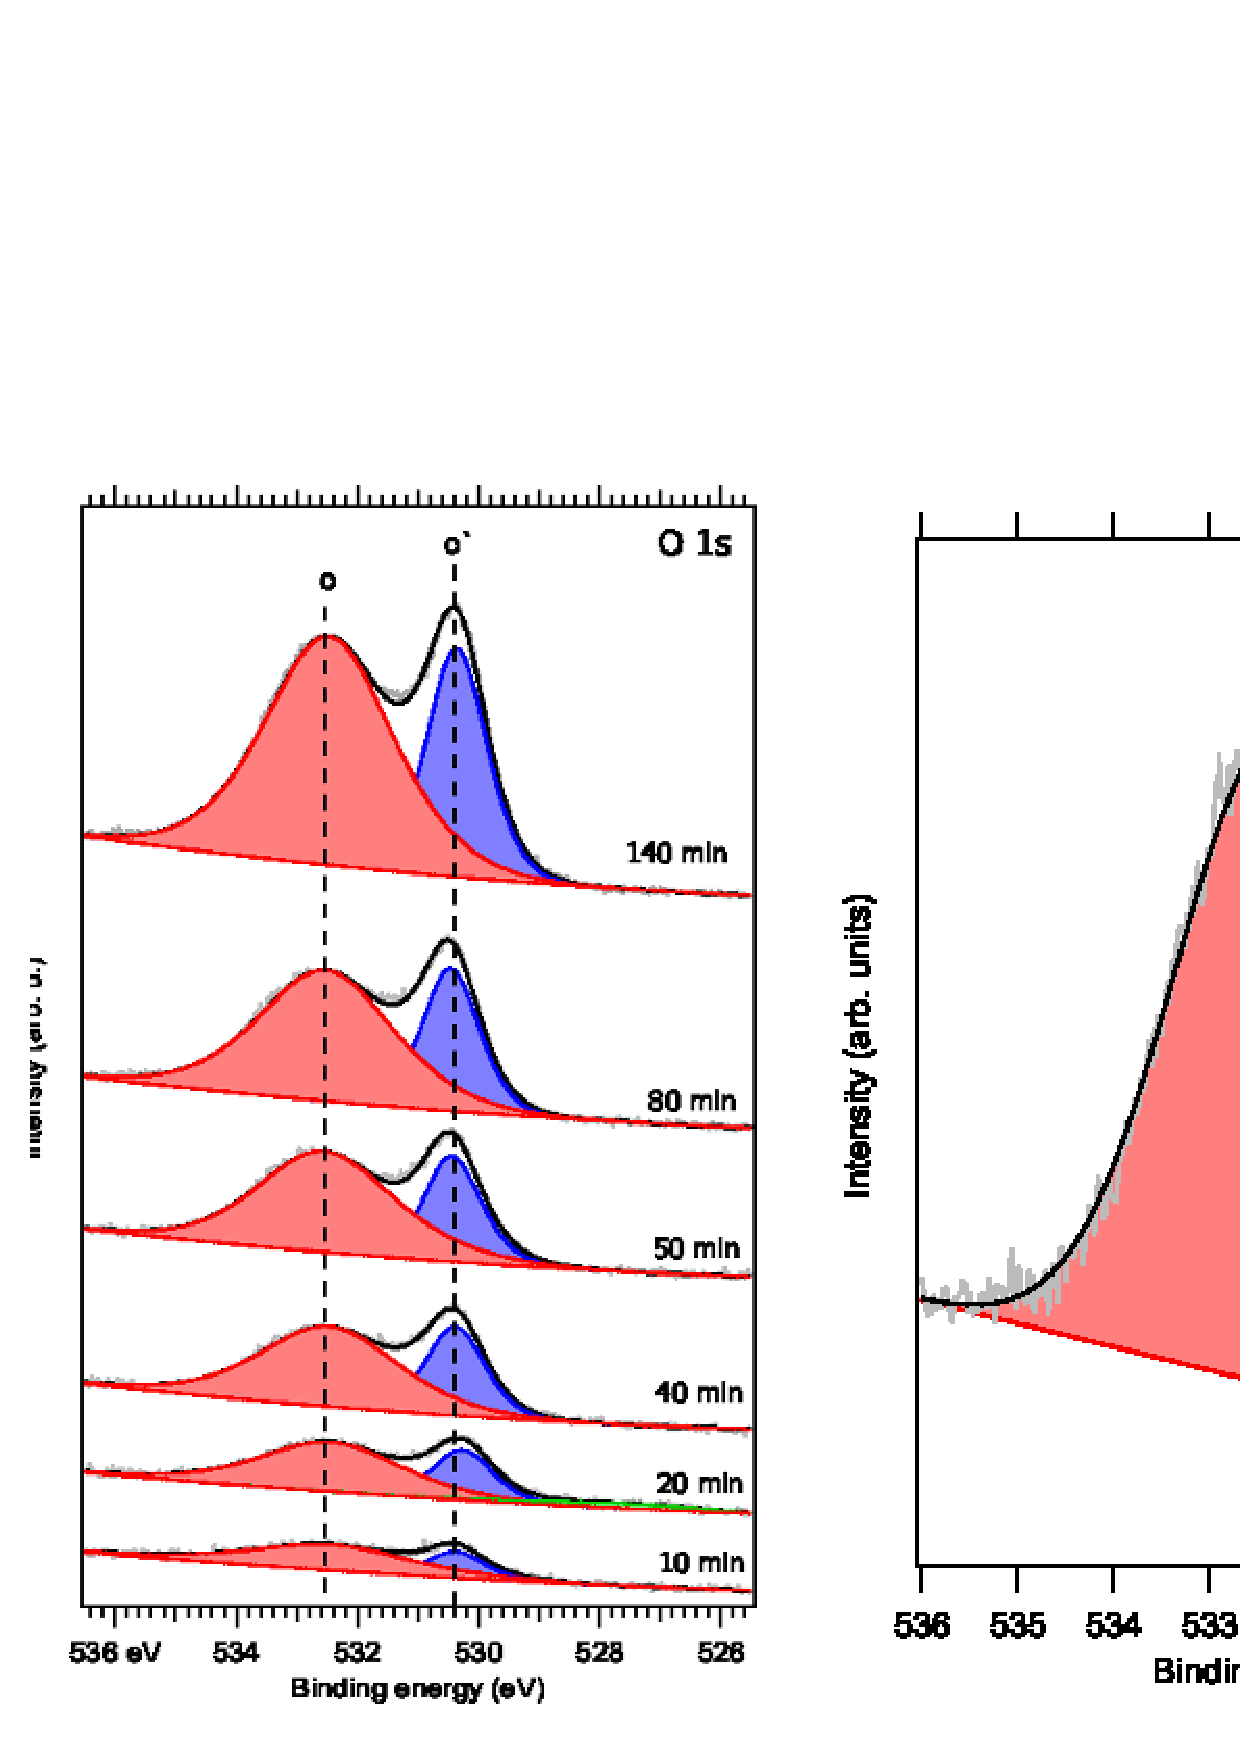
\includegraphics[width=0.7\linewidth]{O1s_all_fits_and_angle55.png}}
		\caption{РФЭС спектры O1s-уровня на разных стадиях экспозиции (a), записанный по нормали к поверхности и пик интенсивности кислорода, записанный при положении анализатора под углом 55\degree к нормали поверхности(b).}
		\label{pic:O1s_all}
	\end{figure}
На рис.~\ref{pic:O1s_all}(a) представлена серия спектров фотоэмиссии кислорода O1s в течение прогрева системы 
h-BN/Co(0001), записанная при положении анализатора по нормали к поверхности. Пик O1s содержит две компоненты: o с энергией связи 532.2 eV и o' с энергией связи 530.3 eV. Оба пика появляются после 10 минут экспозиции и растут в течение всех этапов прогрева образца в кислороде. На рис.~\ref{pic:O1s_all}(b) представлен пик интенсивности кислорода, записанный при положении анализатора под углом 55\degree к нормали поверхности. При скользящем угле выхода фотоэлектронов пик интенсивности o' рис.~\ref{pic:O1s_all}(b) почти в 5 раз меньше пика o, в то время как при выходе фотоэлектронов по нормали к поверхности рис.~\ref{pic:O1s_all}(a), этот пик меньше пика o только в 2 раза. Отсюда можно сделать вывод, что атомы кислорода находятся на разной глубине относительно поверхности системы h-BN/Co(0001), а именно, компонента o относится к атомам кислорода, которые встроились в решетку h-BN, а компонента o' характеризует атомы кислорода, интеркалировавшие под монослой гексагонального нитрида бора. Большая ширина пика o является следствием суперпозиции двух пиков оксидов $\mathrm{BN_2O}$ и $\mathrm{BO_3}$~\cite{Shevelev2019_h-BN/Co_oxydation}. 




\subsection{Анализ спектров поглощения}

Теперь рассмотрим спектры поглощения. После каждого этапа прогрева системы h-BN/Co(0001) вместе с фотоэмиссионными спектрами также снимались спектры NEXAFS. На рис.~\ref{pic:NEXAFS_B_K_edge} представлены B спектры  K-края
	\begin{figure}[!ht]
		\center{\includegraphics[width=0.8\linewidth]{BN_B_K_edge_all_40deg_to_beam.eps}}
		\caption{Спектры поглощения К-края бора.}
		\label{pic:NEXAFS_B_K_edge}
	\end{figure}
поглощения h-BN, соответствующие исходному h-BN/Co(0001) (a), через 10 минут после экспозиции с кислородом (b), 
20 минут (c), 30 минут (d), 40 минут (e), 60 минут (d) и насыщенный кислородом h-BN/Co(0001) после 240 минут экспозиции (f). Пик А соответствует гибридизированным состояниям h-BN-Co. В процессе прогрева интенсивность этого пика заметно понижается, и, после 240 минут прогрева системы, пик А становится практически незаметным. Пик B отвечает за квазисвободный гексагональный нитрид бора~\cite{Huber2015_Oxy_Stab_defffects_in_hBN}. Этот пик становится более острым в процессе прогрева h-BN/Co(0001) в кислороде, что соответствует квазисвободному h-BN и подтверждает интеркаляцию кислорода под монослой нитрида бора~\cite{Makarova2019_h-BN/Ni_Oxydation, Shevelev2019_h-BN/Co_oxydation}. Также следует
обратить внимание на пики $\mathrm{a_1}$, $\mathrm{a_2}$ и $\mathrm{a_3}$ с энергиями связи 192.7 eV, 193.3 eV и 193.9 eV соответственно. В работе \cite{Huber2015_Oxy_Stab_defffects_in_hBN} было показано, что пик $\mathrm{a_1}$ соответствует $\mathrm{BN_2O}$, пик $\mathrm{a_2}$ соответствует $\mathrm{BNO_2}$, а пик $\mathrm{a_3}$ соответствует $\mathrm{BO_3}$. Исходя из интенсивностей пиков $\mathrm{a_1}$, $\mathrm{a_2}$ и $\mathrm{a_3}$ полученного спектра поглощения B K- уровня, можно заключить, что на поверхности гексагонального нитрида бора при прогреве в кислороде преобладает образование структуры $\mathrm{BN_2O}$ в течение всего процесса прогрева. После 240 минут экспозиции также становится явно выраженным пик $\mathrm{a_3}$, что говорит о появлении структуры $\mathrm{BO_3}$ на поверхности 
h-BN/Co(0001). Пик $\mathrm{a_2}$ становится заметным только после 240 минут прогрева. Интенсивность этого пика очень низкая, а значит структуры $\mathrm{BNO_2}$ практически не образуются на поверхности гексагонального нитрида бора при прогреве системы h-BN/Co(0001) в молекулярном кислороде.



\section{Моделирование окисленного нитрида бора}

\subsection{Статистический расчет встраивания атомов кислорода в монослой h-BN}

Для лучшего понимания процесса окисления гексагонального нитрида бора было выполнено моделирование окисленной системы 
h-BN исходя из предположения, что атомы кислорода встраиваются в решетку случайным образом. В процессе моделирования
был построен фрагмент решетки гексагонального нитрида бора 200х200, который содержал 80000 атомов. Атомы азота случайным образом 
заменялись атомами кислорода. Количество атомов кислорода определялось из концентрации кислорода на поверхности в эксперименте. 
Далее были подсчитаны концентрации азота и структур вида $\mathrm{BN_3}$, $\mathrm{BN_2O}$, $\mathrm{BNO_2}$ и $\mathrm{BO_3}$ в 
кристаллической решетке  h-BN.
	\begin{figure}[!ht]
		\center{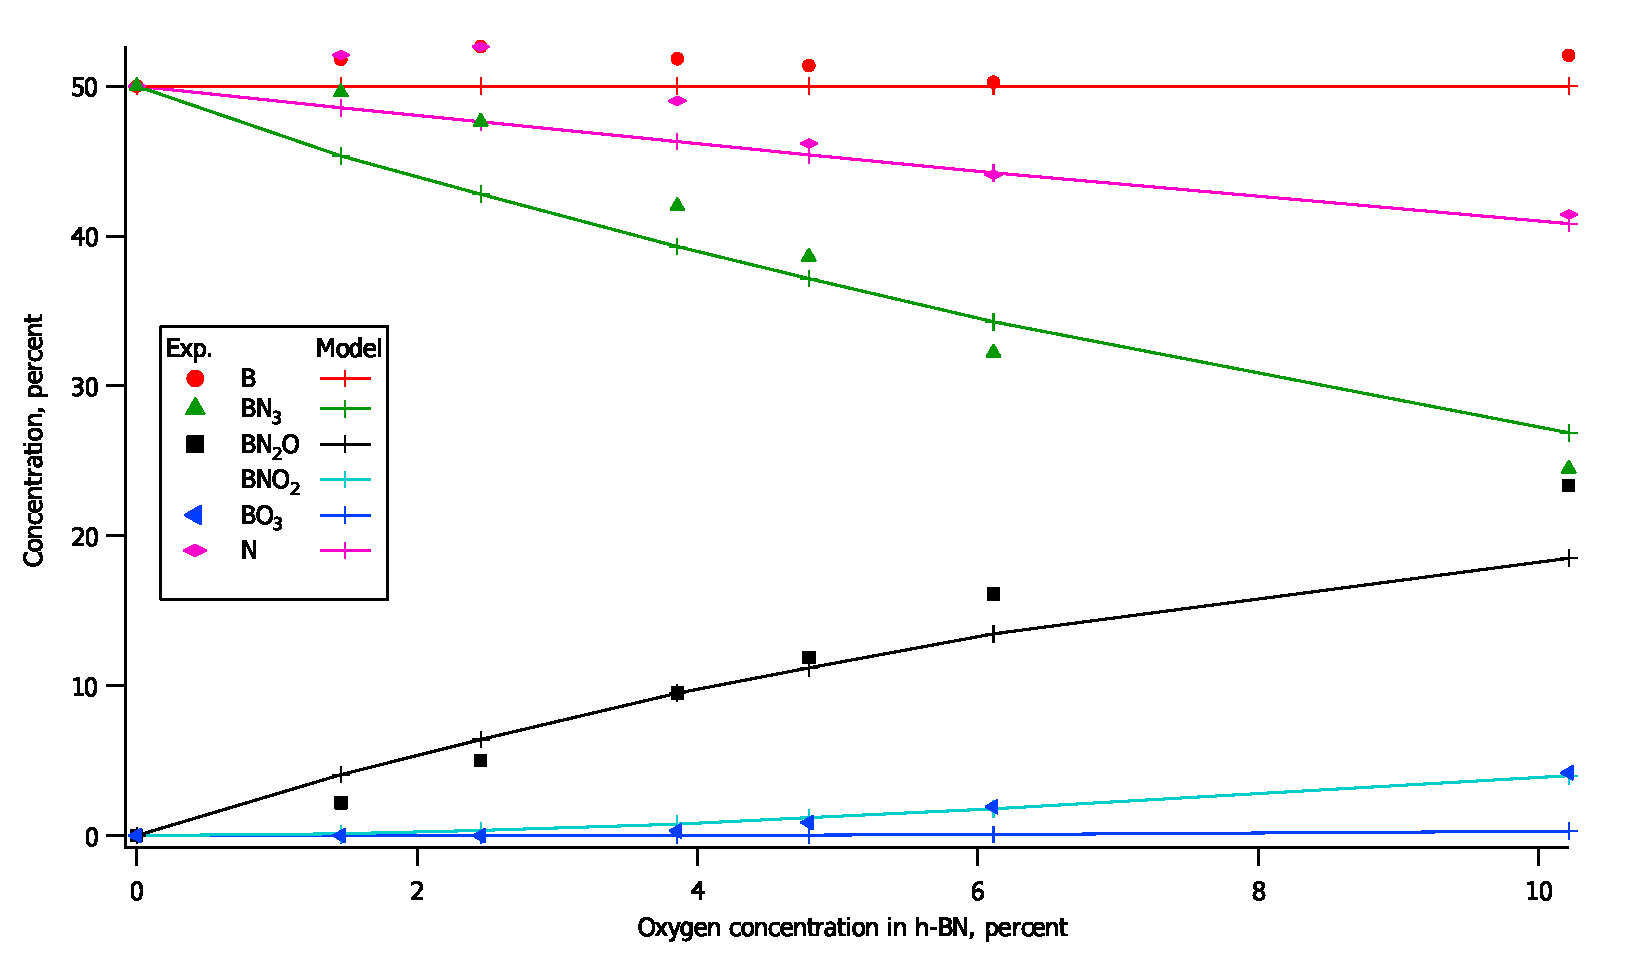
\includegraphics[width=0.8\linewidth]{BN_200x200_experiment_and_model.eps}}
		\caption{Экспериментальные и статистически рассчитанные концентрации азота и бора в зависимости от концентрации кислорода 
		в решетке h-BN.}
		\label{pic:BN_200x200_experiment_and_model}
		\end{figure}
На рис.~\ref{pic:BN_200x200_experiment_and_model} представлены для сравнения экспериментальные и статистически 
рассчитанные концентрации азота и бора в зависимости от концентрации кислорода в решетке h-BN. Из графика видно,
что все модельные кривые концентраций, кроме $\mathrm{BNO_2}$ и $\mathrm{BO_3}$, согласуются с экспериментально полученными 
концентрациями. Из расчета получается, что количество структур  $\mathrm{BNO_2}$, образующихся в результате случайного замещения,
преобладает над структурами $\mathrm{BO_3}$, что отражено на рис.~\ref{pic:BN_200x200_experiment_and_model}. Однако
в эксперименте, как было сказано ранее, структуры вида $\mathrm{BNO_2}$ практически не образовывались на поверхности.
На графике видно, что экспериментальная кривая $\mathrm{BO_3}$ совпадает с модельной кривой $\mathrm{BNO_2}$. Отсюда
можно сделать вывод, что в реальном эксперименте структуры $\mathrm{BNO_2}$ практически не образуются, вместо них
сразу появляются структуры $\mathrm{BO_3}$. 


\subsection{Расчет структуры \textbf{$\mathrm{BNO_2}$}}

Чтобы понять почему структуры вида $\mathrm{BNO_2}$ не образуются в эксперименте, с помощью  теории функционала плотности (DFT) в программе
FPLO(full-potential local-orbital minimum-basis code)~\cite{Koepernik1999} была рассчитана такая структура. Для этого рассмотрена ячейка гексагонального 
нитрида бора в вакууме. Элементарная ячейка содержала встроенные атомы кислорода таким образом, что они образовывали структуру $\mathrm{BNO_2}$. 
\begin{figure}[!ht]
\begin{minipage}[h]{0.49\linewidth}
\center{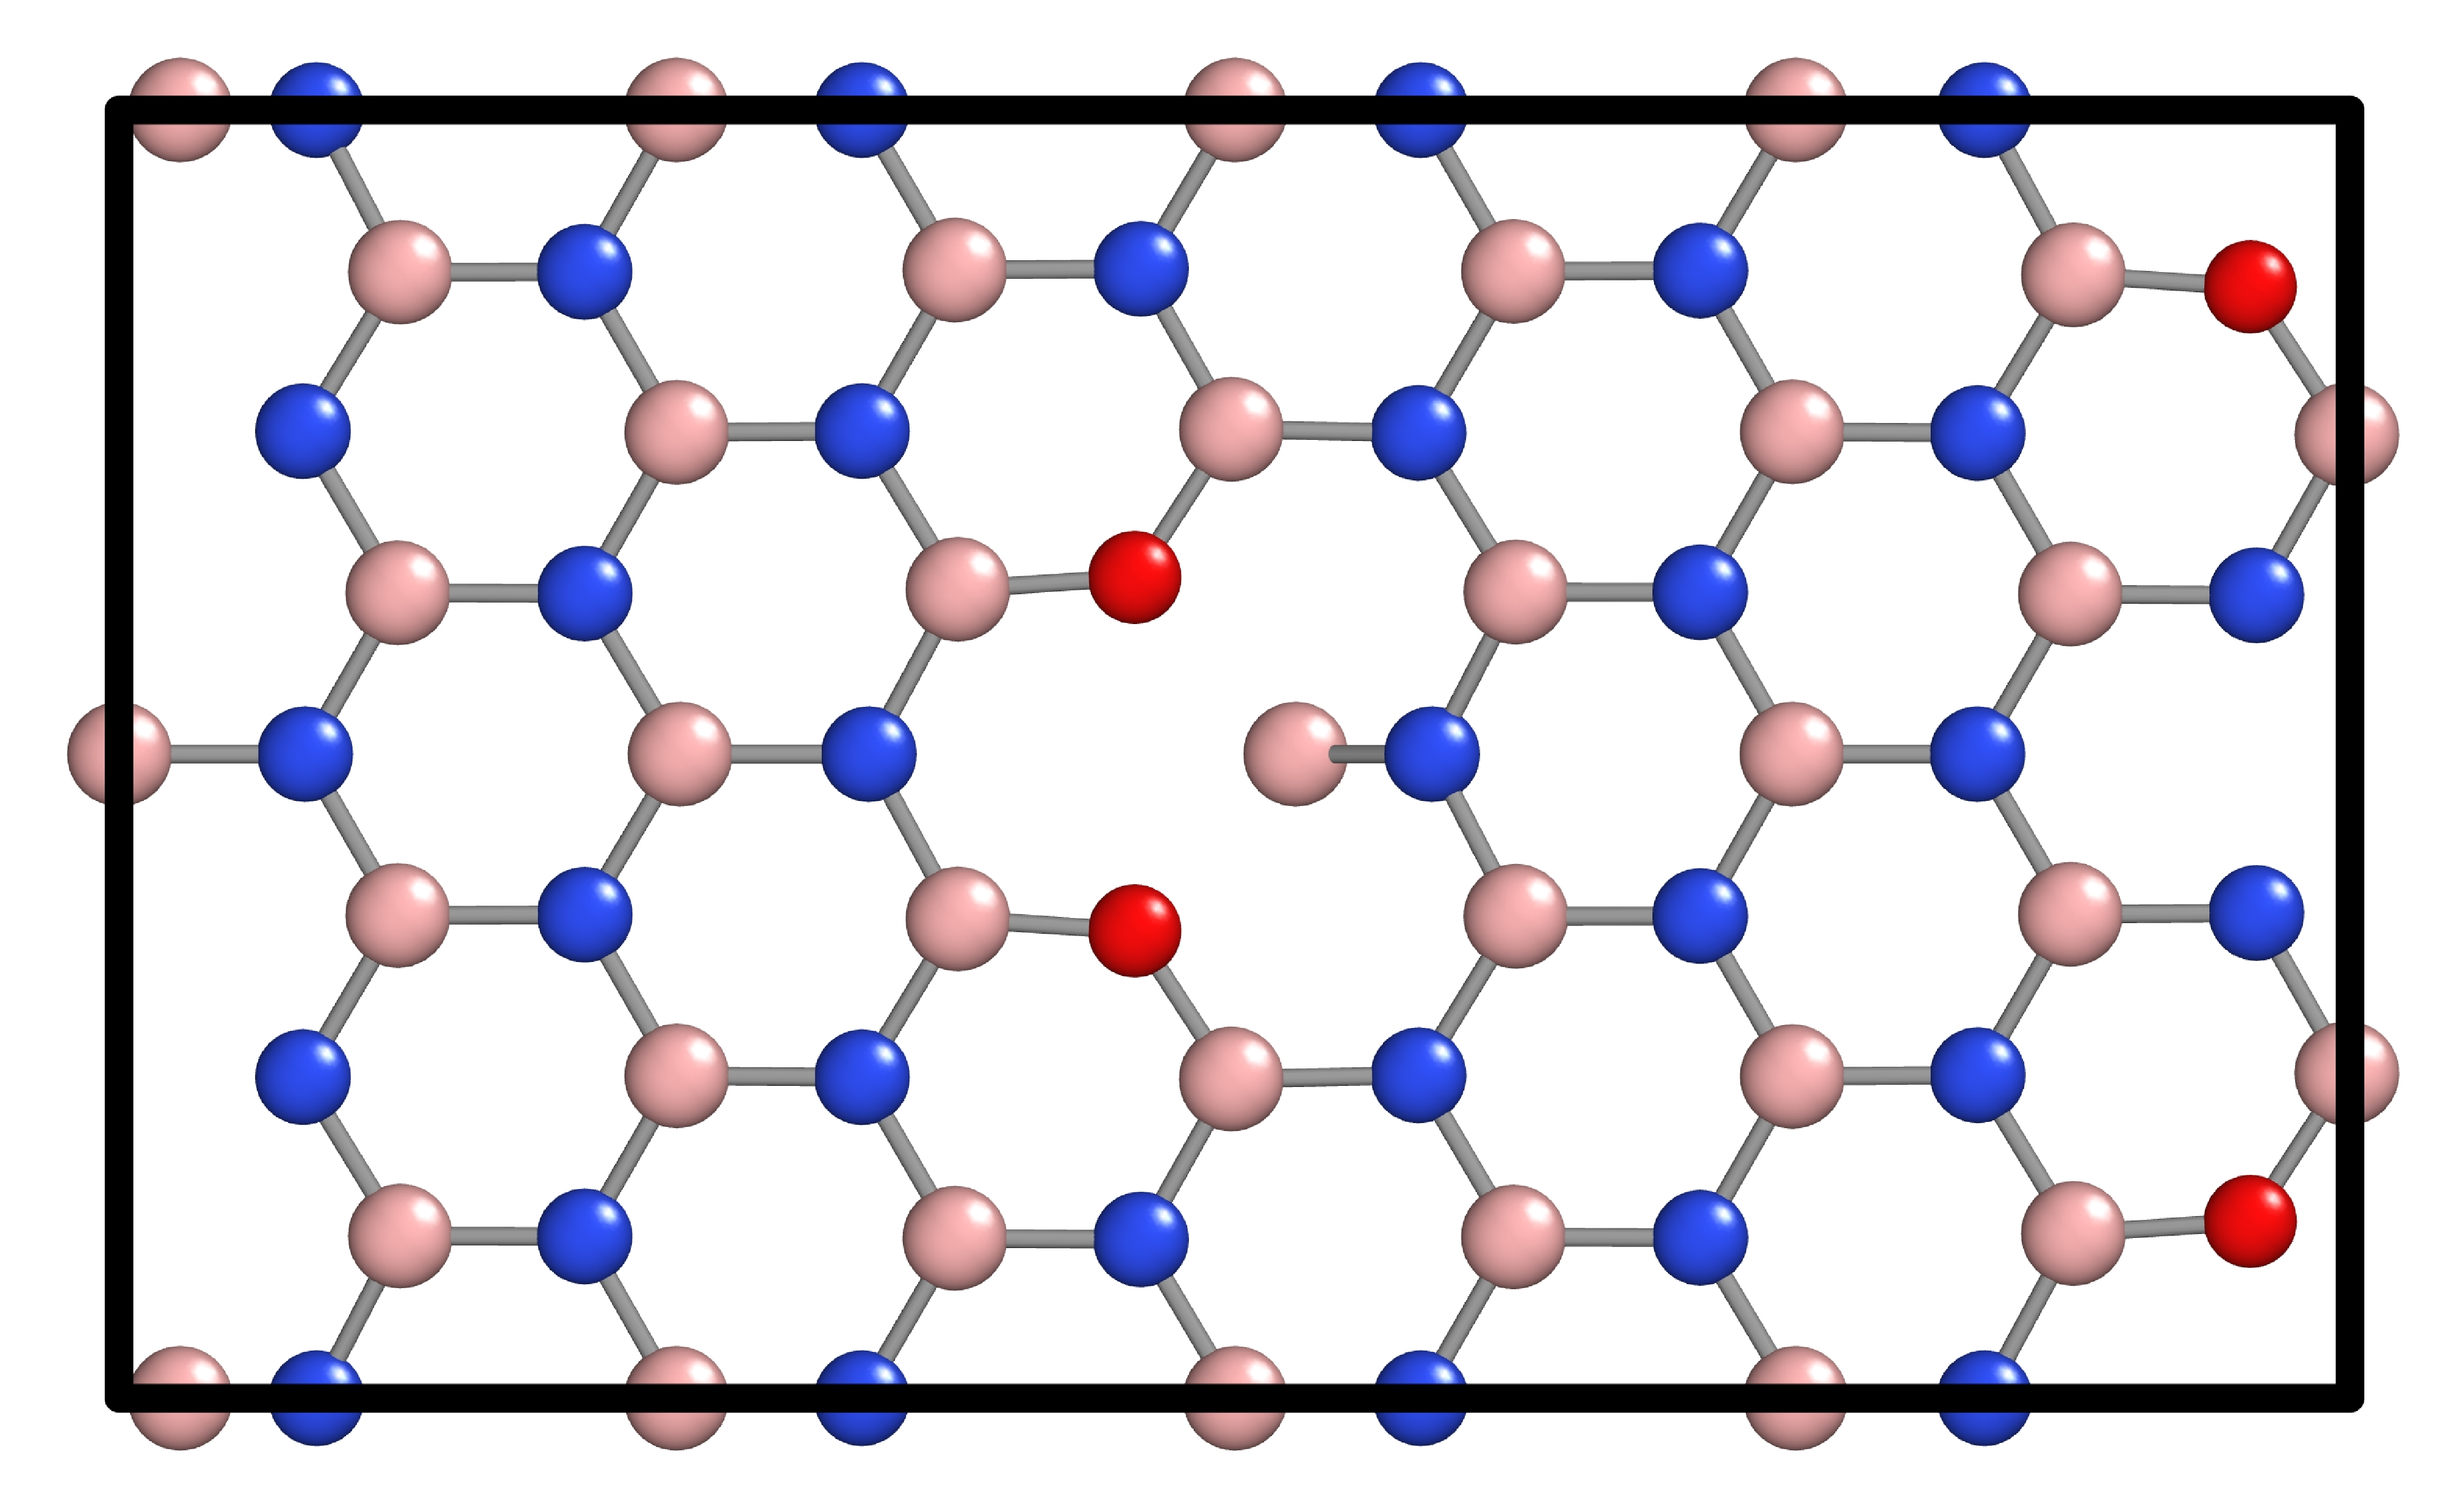
\includegraphics[width=0.9\linewidth]{BNO2_relaxed3.eps} \\ а)}
\end{minipage}
\hfill
\begin{minipage}[!ht]{0.49\linewidth}
\center{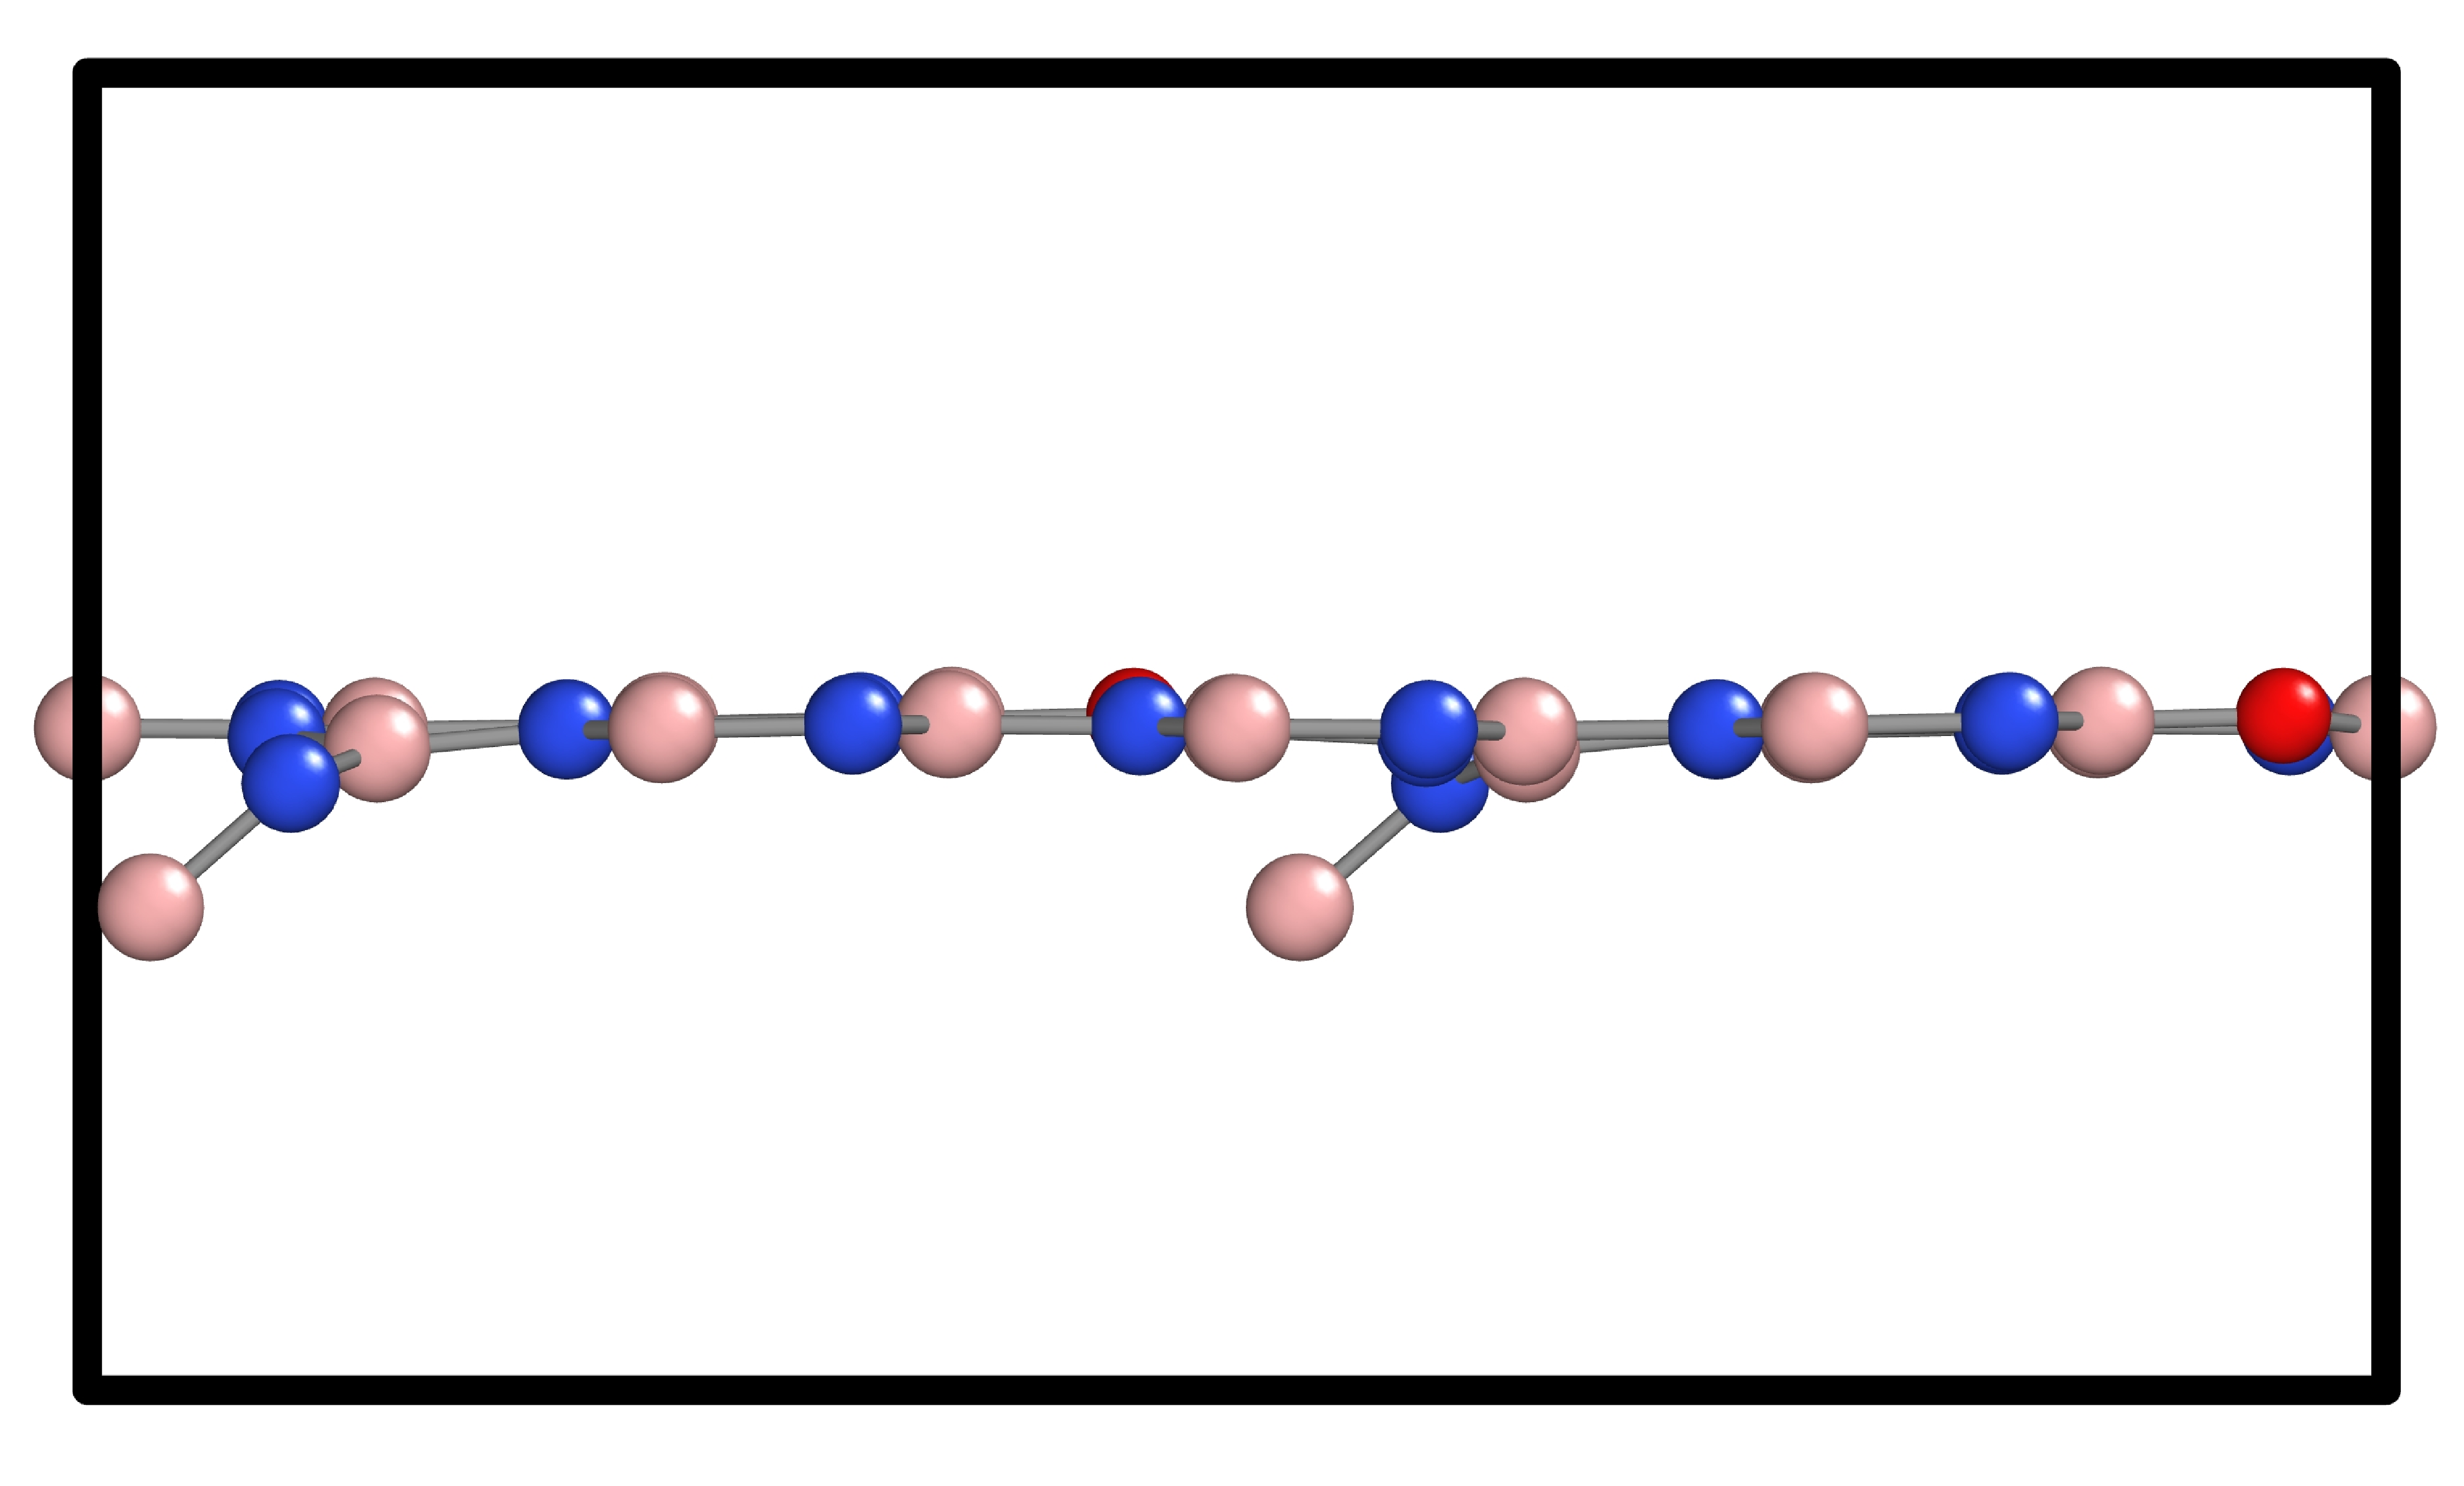
\includegraphics[width=0.9\linewidth]{BNO2_relaxed4.eps} \\ б)}
\end{minipage}
\caption{Рассчитанная структура дефекта $\mathrm{BNO_2}$ в кристаллической решетке h-BN.}
\label{BNO2_relaxed}
\end{figure}
На рис.~\ref{BNO2_relaxed} приведена рассчитанная методом DFT кристаллическая решетка гексагонального нитрида бора 
со встроенными атомами кислорода. 
Релаксация такой системы показала, что расстояние от атома бора до соседних атомов кислорода равняется b=2.37~\AA~рис.~\ref{pic:BNO2_B_height}. В работе~\cite{Coulson1968} показано, что в химических соединениях длина связи $\mathrm{B-O}$ варьируется в 
диапазоне значений от 1.205~\AA~до 1.35~\AA. Расстояние b рис.~\ref{pic:BNO2_B_height}, как показал расчет, 
оказывается больше максимально возможного на 1~\AA. Это означает, что бор не образует связи с кислородами, а 
структура $\mathrm{BNO_2}$ является неустойчивой. Этот расчет говорит о том, что структуры вида $\mathrm{BNO_2}$ 
оказываются нестабильными. Это и является причиной отсутствия $\mathrm{BNO_2}$ в эксперименте.
\begin{figure}[!ht]
\center{\includegraphics[width=0.6\linewidth]{BNO2_B_height.png}}
\caption{Рассчитанная методом DFT структура $\mathrm{BNO_2}$.}
\label{pic:BNO2_B_height}
\end{figure}



\clearpage
